\documentclass[11pt,a4paper]{article}

\usepackage[margin=2cm]{geometry}
\usepackage{parskip}
\usepackage{amsmath}
\usepackage{enumitem}
\usepackage{multicol}
\usepackage{booktabs}
\usepackage{graphicx}
\usepackage{amssymb}



\setlist[itemize]{leftmargin=1.2em}
\setlist[enumerate]{leftmargin=1.2em,label=\arabic*.}

\newcommand{\imgbox}[2][5cm]{%
  \fbox{%
    \begin{minipage}[c][#1][c]{\linewidth}
    \centering #2
    \end{minipage}
  }%
}

\begin{document}

\begin{center}
  {\LARGE \textbf{Models of the Atom}}\\[2mm]
  \normalsize Name:\rule{0.4\linewidth}{0.4pt}\hfill Date:\rule{0.25\linewidth}{0.4pt}
\end{center}

\section*{1) A brief history of the atom}
The idea that matter is made of indivisible particles goes back to ancient Greece: around 400~BC, \textbf{Democritus} coined the term \emph{atomos}, meaning ``uncuttable'', to describe the smallest possible units of matter. For centuries this was a philosophical idea rather than a scientific theory.  

By the 1800s, chemists had begun to find patterns in the behaviour of substances. \textbf{John Dalton} proposed an early atomic theory (1803), suggesting that elements are made of tiny particles which combine in simple ratios. Later in the century, \textbf{Dmitri Mendeleev} arranged the known elements into his \emph{periodic table} (1869), recognising repeating trends in their chemical properties and leaving gaps for elements yet to be discovered.  

A major leap came in 1897 when \textbf{J.\,J.\ Thomson} discovered the electron and proposed the \emph{plum pudding model}, in which negative electrons were embedded in a diffuse positive ``pudding''. Between 1909 and 1911, \textbf{Geiger and Marsden}, working under \textbf{Ernest Rutherford}, carried out the famous gold foil scattering experiment. Rutherford (1911) interpreted their results as evidence for a tiny, dense, positively charged \emph{nucleus}, giving rise to the \emph{nuclear model} (sometimes called the ``solar system'' model).  

In 1913, \textbf{Niels Bohr} refined this picture by proposing that electrons move in \emph{quantised orbits}, explaining observed patterns in atomic spectra. Finally, in 1932, \textbf{James Chadwick} discovered the neutron, completing the modern picture of the atom: a dense nucleus of protons and neutrons with electrons arranged in shells around it.


\section*{2) From \emph{plum pudding} to \emph{nuclear} (solar system) model}
\subsection*{(a) The plum pudding model}
Main features (as understood c.\,1904):
\begin{itemize}
  \item Mass and positive charge spread evenly throughout the atom (no central nucleus).
  \item Electrons are embedded within this positive ``mass/charge'' like plums in a pudding.
  \item Atom treated as a continuous, largely solid distribution rather than mostly empty space.
\end{itemize}

\begin{figure}[h]
  \centering
  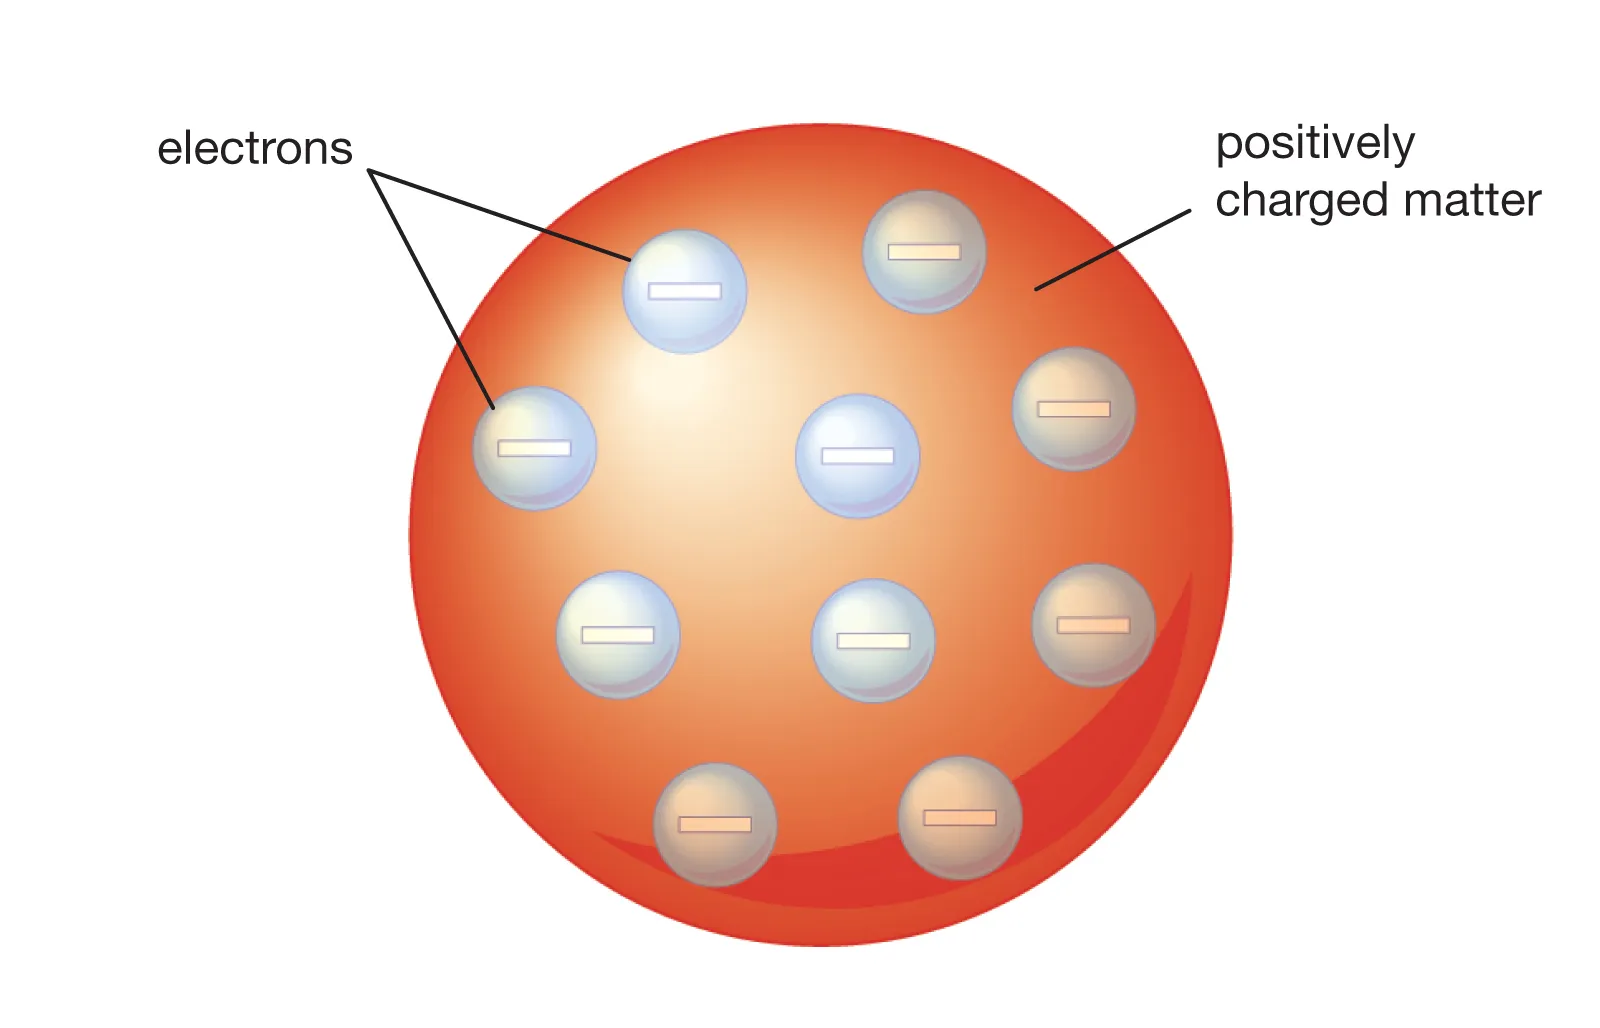
\includegraphics[width=0.5\linewidth]{img1.png}
  \caption{plum pudding model}
  \label{fig:img1}
\end{figure}

\newpage

\subsection*{(b) The gold foil (alpha scattering) experiment}
\textbf{Method:} A beam of alpha particles (He nuclei) was directed at very thin gold foil; a screen detected their scattering angles.\\
\textbf{Key observations:}
\begin{itemize}
  \item Most alpha particles passed straight through with no deflection.
  \item Some were deflected by small angles.
  \item A very small fraction were deflected through large angles, some nearly straight back.
\end{itemize}
\textbf{Conclusions:}
\begin{itemize}
  \item Positive charge and almost all the mass are concentrated in a tiny central nucleus.
  \item The atom is mainly empty space.
  \item Electrons are not embedded throughout a solid mass; they are some distance from the centre.
\end{itemize}

\begin{figure}[h]
  \centering
  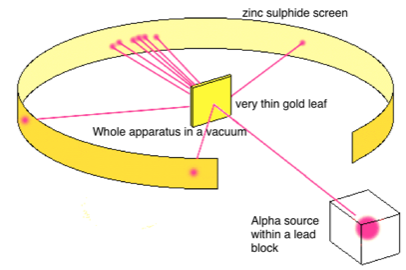
\includegraphics[width=0.6\linewidth]{img2.png}
  \caption{gold foil experiment}
  \label{fig:img2}
\end{figure}

\newpage

\subsection*{(c) The nuclear (solar system) model}
\begin{itemize}
  \item A tiny, dense nucleus at the centre contains the positive charge and most of the mass.
  \item Electrons orbit the nucleus some distance away.
  \item The atom is mostly empty space.
\end{itemize}

\begin{figure}[h]
  \centering
  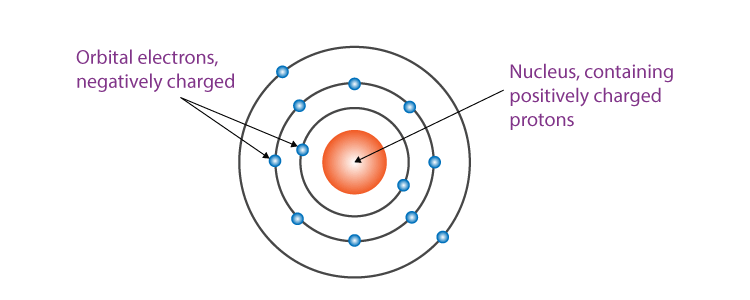
\includegraphics[width=0.8\linewidth]{img3.png}
  \caption{solar system model}
  \label{fig:img3}
\end{figure}

\paragraph{Differences between the plum pudding and nuclear models:}
\begin{itemize}
  \item \textbf{Mass:}
    \begin{itemize}
      \item Plum pudding $\rightarrow$ mass evenly distributed
      \item Nuclear model $\rightarrow$ mass concentrated at centre (nucleus)
    \end{itemize}

  \item \textbf{Positive charge:}
    \begin{itemize}
      \item Plum pudding $\rightarrow$ positive charge spread throughout
      \item Nuclear model $\rightarrow$ positive charge in small central nucleus
    \end{itemize}

  \item \textbf{Electrons:}
    \begin{itemize}
      \item Plum pudding $\rightarrow$ electrons embedded in the positive mass
      \item Nuclear model $\rightarrow$ electrons orbit some distance from nucleus
    \end{itemize}

  \item \textbf{Space:}
    \begin{itemize}
      \item Plum pudding $\rightarrow$ treated as a solid/continuous mass
      \item Nuclear model $\rightarrow$ atom mainly empty space
    \end{itemize}
\end{itemize}


\newpage
\section*{3) The current model (with neutrons)}
\begin{itemize}
  \item Nucleus contains \textbf{protons} (charge $+1$) and \textbf{neutrons} (charge $0$).
  \item \textbf{Electrons} (charge $-1$) occupy shells/energy levels around the nucleus.
\end{itemize}

\begin{figure}[h]
  \centering
  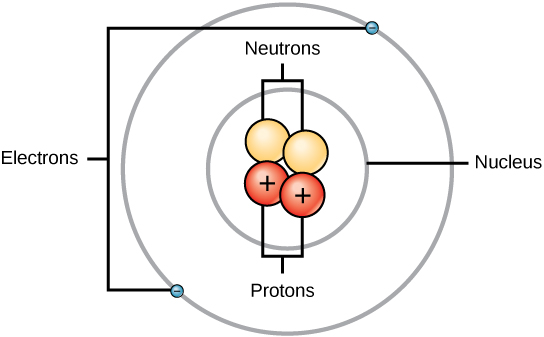
\includegraphics[width=0.5\linewidth]{img4.png}
  \caption{current atomic model}
  \label{fig:img4}
\end{figure}

\paragraph{Atomic numbers and simple formulae}
Let atomic number $Z=$ number of protons; mass number $A=$ protons $+$ neutrons.
\[
\text{No.\ of protons} = Z \qquad
\text{No.\ of electrons (neutral atom)} = Z \qquad
\text{No.\ of neutrons} = A - Z
\]

\newpage
\section*{4) Questions}
\subsection*{A. History of the atom}
\begin{enumerate}
  \item Who proposed the plum pudding model, and in which decade?
  \item What were the three key observations from the gold foil experiment?
  \item Which observations contradict the plum pudding model? Explain briefly.
  \item What two main conclusions about atomic structure came from the large-angle deflections?
  \item Who discovered the neutron, and why did that matter for the nuclear model?
\end{enumerate}

\subsection*{B. Model overviews}
\begin{enumerate}[resume]
  \item List \textbf{two} features of the plum pudding model.
  \item List \textbf{two} features of the nuclear (solar system) model.
  \item Complete the table by ticking the model(s) that match each statement:

  \vspace{2mm}
  \begin{tabular}{@{}p{0.55\linewidth}cc@{}}
    \toprule
    Statement & Plum pudding & Nuclear \\
    \midrule
    Mass concentrated at the centre & \(\square\) & \(\square\) \\
    Positive charge spread throughout the atom & \(\square\) & \(\square\) \\
    Electrons embedded in positive mass & \(\square\) & \(\square\) \\
    Atom mainly empty space & \(\square\) & \(\square\) \\
    \bottomrule
  \end{tabular}
\end{enumerate}

\subsection*{C. Compare the two models}
\begin{enumerate}[resume]
  \item Describe how the location of \textbf{mass} differs between the two models.
  \item Describe how the \textbf{positive charge} is arranged in each model.
  \item Describe where the \textbf{electrons} are in each model.
  \item Explain how the gold foil experiment led to rejecting the plum pudding model.
\end{enumerate}

\subsection*{D. Structure and key terms (GCSE)}
\begin{enumerate}[resume]
  \item Define: \textbf{atomic number} ($Z$) and \textbf{mass number} ($A$).
  \item Define: \textbf{isotope}.
  \item State the relative charges of proton, neutron, and electron.
  \item In a \emph{neutral} atom, how do the numbers of protons and electrons compare?
  \item Why is almost all the mass of an atom in the nucleus?
\end{enumerate}

\newpage
\subsection*{E. Counting protons, neutrons, electrons}
For each neutral atom below, fill in the table.
\[
\text{No.\ of protons} = Z,\quad
\text{No.\ of neutrons} = A-Z,\quad
\text{No.\ of electrons} = Z
\]

\begin{center}
\begin{tabular}{@{}lccccc@{}}
\toprule
Atom & $A$ & $Z$ & No.\ of protons & No.\ of neutrons & No.\ of electrons \\
\midrule
Helium-4      & 4  & 2  & \rule{1cm}{0.4pt} & \rule{1cm}{0.4pt} & \rule{1cm}{0.4pt} \\
Carbon-12     & 12 & 6  & \rule{1cm}{0.4pt} & \rule{1cm}{0.4pt} & \rule{1cm}{0.4pt} \\
Nitrogen-14   & 14 & 7  & \rule{1cm}{0.4pt} & \rule{1cm}{0.4pt} & \rule{1cm}{0.4pt} \\
Oxygen-16     & 16 & 8  & \rule{1cm}{0.4pt} & \rule{1cm}{0.4pt} & \rule{1cm}{0.4pt} \\
Sodium-23     & 23 & 11 & \rule{1cm}{0.4pt} & \rule{1cm}{0.4pt} & \rule{1cm}{0.4pt} \\
Chlorine-35   & 35 & 17 & \rule{1cm}{0.4pt} & \rule{1cm}{0.4pt} & \rule{1cm}{0.4pt} \\
\bottomrule
\end{tabular}
\end{center}

\subsection*{F. Quick applications}
\begin{enumerate}[resume]
  \item An atom has $Z=12$ and $A=24$. Find the numbers of p, n, e.
  \item An atom has 20 protons and 20 neutrons. State $A$ and $Z$, and give p, n, e.
  \item Magnesium has $Z=12$. Two isotopes have $A=24$ and $A=25$. For each isotope, give p, n, e (neutral atoms).
  \item Why do isotopes of the same element have nearly identical chemical properties?
\end{enumerate}

\vfill
\hrule
\small \textit{Tip:} In neutral atoms, electrons $=$ protons. Neutrons $=A-Z$. Large-angle alpha deflections $\Rightarrow$ tiny, massive, positively charged nucleus.

\end{document}
